\documentclass[12pt]{article}
\usepackage[utf8]{inputenc}
\usepackage{amsmath}
\usepackage{amssymb}
\usepackage{amsfonts}
\usepackage[polish]{babel}
\usepackage[OT4]{fontenc}
\usepackage{graphicx}
\usepackage{caption}
\usepackage{subcaption}
\usepackage{adjustbox}
\usepackage{float}
\usepackage{colortbl}
\definecolor{color1}{RGB}{164, 116, 219}
\definecolor{color2}{RGB}{232, 212, 132}


\captionsetup[table]{name=Tabela}
\graphicspath{{./images}}

\textheight 23.2 cm

\textwidth 6.0 in

\hoffset = -0.5 in

\voffset = -2.4 cm


\begin{document}

%h�?
%\thispagestyle{empty}

\vspace*{3ex}
\begin{flushright}
{\large 28 listopada 2021}
\end{flushright}

\begin{flushleft}
{\large Przemys\l aw Kacprzak\\
Grupa 4a}
\end{flushleft}

\hskip3cm

\begin{center}

\Large {\bf 24. Obliczanie ca\l ek $\iint_D f(x,y)dxdy $ \\ 
    na obszarze $D = \{(x,y) \in \mathbb R^2 : |x| + |y| \leq 1\}$ \\
    przez transformację na kwadrat $[-1,1] \times [-1,1]$ \\
    i zastosowanie z\l o\.zonych kwadratur Simsona ze względu na ka\.zdą zmienną}

\vskip2ex
\tableofcontents

\end{center}

\vskip20ex

\newpage
\section{Wstęp}
Obliczenie ca\l ki podw\'ojnej funkcji dw\'och zmiennych na obszarze nie 
będącym prostokątem lub tr\'ojkątem jest zadaniem wymagającym dw\'och czę\'sci:
transformacji obszaru ca\l kowania oraz u\.zycia kwadratury do przybli\.zenia 
wyniku.\\ \\
W raporcie zbadano czy zwiększenie ilo\'sci podprzedzia\l \'ow prowadzi do mniejszych b\l ęd\'ow w 
obliczeniach, oraz w jakim tempie b\l ędy te maleją. Sprawdzono r\'ownie\.z, czy dla wielomian\'ow stopnia 
mniejszego ni\.z 4 b\l ąd maleje wraz z ilo\'scią przedzia\l \'ow. Wykonano tak\.ze eksperyment
polegający na sprawdzeniu dzia\l ania tranformacji obszaru. \\ \\
Por\'ownano tak\.ze dzia\l anie programu z bli\'zniaczą funkcją u\.zywającą kwadratury trapez\'ow.

\section{Opis u\.zytej metody}
Metodą u\.zytą w programie jest przekszta\l cenie obszaru ca\l kowania przy pomocy
macierzy Jakobiego oraz zastosowanie z\l o\.zonych kwadratur Simpsona.\\
Na poni\.zszych wykresach przedstawione są 2 obszary: \\
\begin{figure}[h]
	\centering
	\begin{subfigure}[h]{0.49\linewidth}
		\centering
		\begin{adjustbox}{width=\linewidth}
            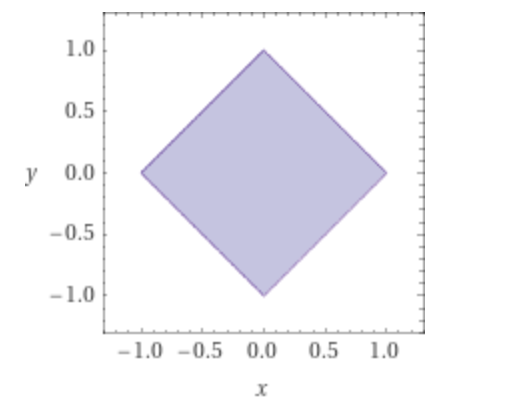
\includegraphics[width=2cm]{wolf_romb.png}
		\end{adjustbox}
            \caption{Obszar D}
	\end{subfigure}
	\hfill
	\begin{subfigure}[h]{0.49\linewidth}
		\centering
		\begin{adjustbox}{width=0.9\linewidth}
            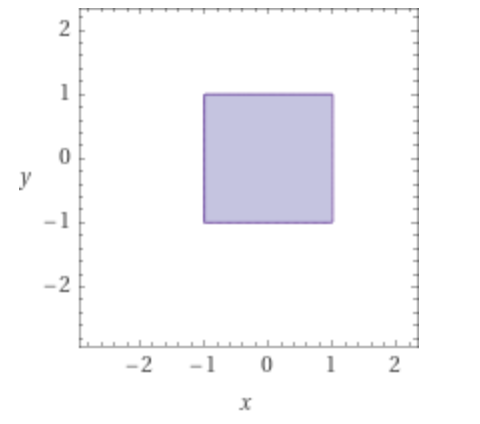
\includegraphics[width=2cm]{wolf_kwad.png}
		\end{adjustbox}
            \caption{Obszar E}
	\end{subfigure}
\end{figure}
$D = \{(x,y) \in \mathbb R^2 : |x| + |y| \leq 1 \}$ oraz $E = [-1,1] \times [-1,1]$.\\
Aby otrzyma\'c obszar E z obszaru D nale\.zy obr\'oci\'c obszar o 45 stopni,
przeciwnie do ruchu wskaz\'owek zegara oraz pomniejszy\'c obszar $\sqrt{2}$ razy.
Czyli nasze funkcje przekszta\l cające będą mia\l y posta\'c
\begin{equation}
    \phi(x,y) = \frac{x+y}{2} \hskip3ex
    \psi(x,y) = \frac{y-x}{2}.
\end{equation}
Wtedy:
\begin{equation}
    D = \{ (u,v): u=\phi(x,y), v=\psi(x,y), (x,y)\in E \}.
\end{equation}
Macierz Jakobiego będzie mia\l a posta\'c
\begin{equation}
    J(x,y) = J_{\phi ,\psi}(x,y) = 
    \left[ \begin{array}{cc}
        \frac{\delta \phi}{\delta x}(x,y) & \frac{\delta \phi}{\delta y}(x,y) \\
        \frac{\delta \psi}{\delta x}(x,y) & \frac{\delta \psi}{\delta y}(x,y) 
    \end{array}\right] =
    \left[ \begin{array}{cc}
        \frac{1}{2} & \frac{1}{2} \\
        -\frac{1}{2} & -\frac{1}{2} 
    \end{array}\right] .
\end{equation}
Zatem Jakobian to $ \frac{1}{2}$.\\
Obliczymy wiec ca\l kę
\begin{equation}
    \iint_E f(\phi(x,y),\psi(x,y))\frac{1}{2}.
\end{equation}
U\.zyjemy do tego z\l o\.zonych kwadratur Simpsona ze względu na ka\.zdą zmienną.
Kwadratura prosta Simpsona dla przedzia\l u $[a,b]$ polega na pobraniu warto\'sci
funkcji dla punkt\'ow $a,\frac{a+b}{2},b$ i skorzystania ze wzoru
\begin{equation}
    S(f) = \frac{b-a}{6} ( f(a)+4f(\frac{a+b}{2})+f(b) )
\end{equation}
Metoda z\l o\.zona polega na wykonaniu tej operacji dla większej liczby przedzia\l \'ow
i zsumowaniu wynik\'ow. W naszym przypadku dzia\l amy na funkcji 2 zmiennych, więc 
wykonujemy metodę na siatce $n \times m$ gdzie $n$ i $m$ to odpowiednio ilo\'s\'c
podprzedzia\l \'ow, na kt\'ore dzielimy nasz obszar $E$ po osi $x$ i $y$.
\section{Opis eksperyment\'ow}
\subsection{Test transformacji przedzia\l u ca\l kowania}
Poni\.zej pokazany jest wykres przedstawiający obszar [-1,1]x[-1,1]. 
\begin{figure}[!h]
    \centering
    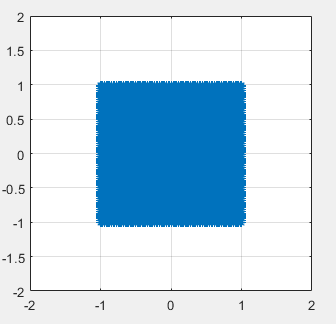
\includegraphics[width=6.8cm]{kwad.png}
    \caption{$[-1,1]\times[-1,1]$ wygenerowany w programie Matlab}
\end{figure}

Zosta\l \ on otrzymany poprzez narysowanie r\'owno roz\l o\.zonych punkt\'ow po tym obszarze.
Teraz przekszta\l cimy ka\.zdy z tych punk\'ow za pomocą przekszta\l cenia z programu i por\'ownamy obszary.\\
\begin{figure}[H]
    \centering
    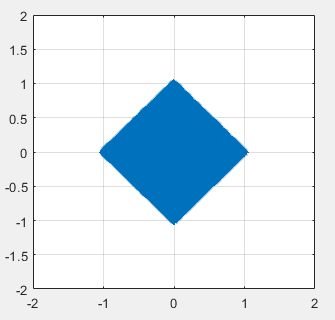
\includegraphics[width=5.5cm]{romb.png}
    \caption{$[-1,1]\times[-1,1]$ po przeksztauceniu za pomocą $\phi $ oraz $\psi$.}
\end{figure}

Jak wida\'c poni\.zszy obszar to $\{(x,y) \in \mathbb R^2 : |x| + |y| \leq 1\}$, co pokazuje poprawno\'s\'c
przekszta\l cenia.
\subsection{Test b\l ęd\'ow dla wielomian\'ow maksymalnie trzeciego stopnia}
Do testu tego u\.zyto trzech losowo wygenerowanych wielomian\'ow stopni: 1, 2, 3.
Dla ka\.zdego z nich obliczano wynik ca\l kowania przy u\.zyciu rosnącej ilo\'sci podprzedzia\l \'ow.
Poni\.zszy wykres przedstawia b\l ędy przy ca\l kowaniu tych funkcji.\\
\begin{figure}[H]
    \centering
    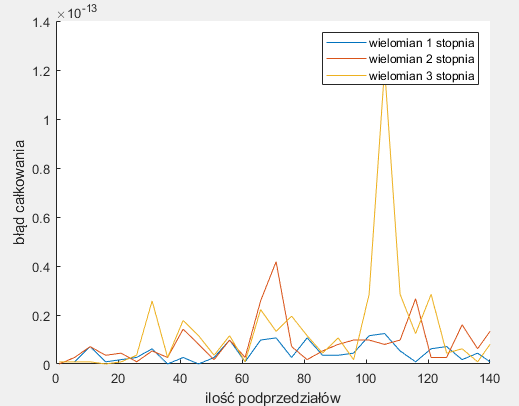
\includegraphics[width=7cm]{less_4.png}
    \caption{B\l ędy dla rosnącej liczby podprzedzia\l \'ow dla wielomian\'ow 
    stopnia niewiększego ni\.z 4.}
\end{figure}
Jak wida\'c b\l ąd nie maleje wraz z ilo\'scią przedzia\l \'ow co pokazuje,
\.ze program jest u\.zyteczny do liczenia ca\l ek z wielomian\'ow stopnia
mniejszego ni\.z 4 oraz, \.ze optymalne przy liczeniu tych wielomian\'ow
jest u\.zywanie tylko jednego podprzedzia\l u. Powy\.zszy wykres pokazuje 
r\'owie\.z, \.ze kwadratura Simpsona jest co najmniej czwartego rzędu.
\newpage
\subsection{Por\'ownanie b\l ęd\'ow dla kwadratury trapez\'ow i Simpsona}
Na poni\.zszych 2 wykresach widzimy b\l ędy ca\l kowania 2 funkcji. 
Na obu wykresach widoczne są 2 krzywe gdzie jedna oznacza b\l ąd przy liczeniu 
ca\l ki przy pomocy kwadratury trapez\'ow a druga przy pomocy kwadratury Simpsona.

\begin{figure}[H]
    \centering
    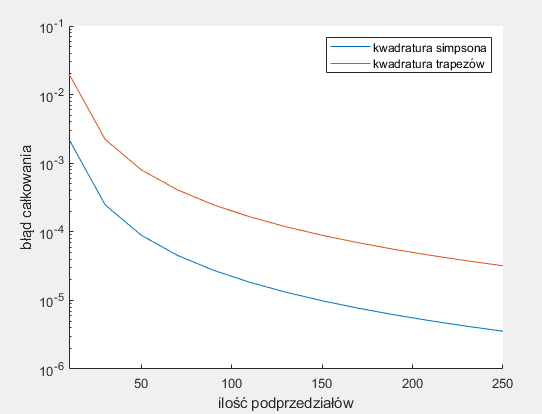
\includegraphics[width=8cm]{trapez_vs_simpson.png}
    \caption{B\l ąd ca\l kowania dla rosnącej liczby podprzedzia\l \'ow
    dla kwadratury trapez\'ow oraz Simpsona}
\end{figure}
Kwadratura trapez\'ow osiąga większe warto\'sci b\l ęd\'ow, co potwierdza to,
\.ze jest kwadraturą mniejszego rzędu ni\.z kwadratura Simpsona. Co więcej
wida\'c, \.ze b\l ędy dla kwadratury trapez\'ow są w przybli\.zeniu 10 razy 
większe, co pokazuje, \.ze kwadratury te r\'o\.znią się dok\l adnie jednym
rzędem. Poni\.zej znajduje się wykres przedstawiający czas oblicze\'n
funkcji dla r\'o\.znych ilo\'sci podprzedzia\l \'ow.
\begin{figure}[H]
    \centering
    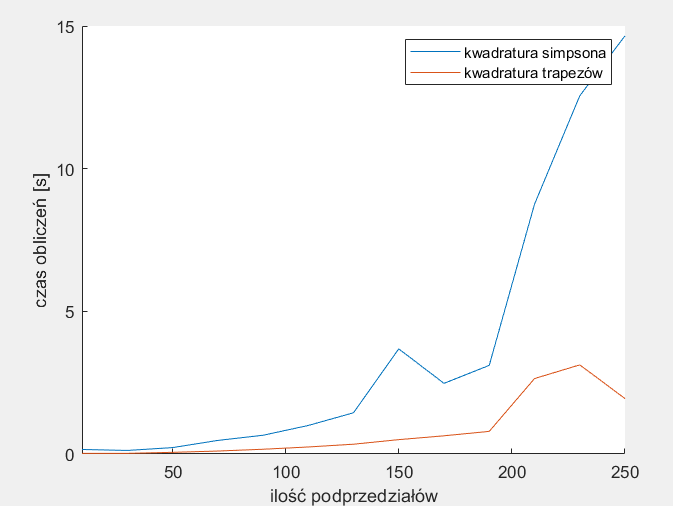
\includegraphics[width=8cm]{time.png}
    \caption{Czas oblicze\'n dla rosnącej ilo\'sci podprzedzia\l \'ow
    przy u\.zyciu kwadratury Simpsona i Trapez\'ow.}
\end{figure}
Jak wida\'c ceną za wiąkszą dok\l adno\'s\'c jest wyd\l u\.zony czas oblicze\'n.



\subsection{Test b\l ęd\'ow dla rosnącej ilo\'sci podprzedzia\l \'ow}
Do testu tego wykorzystano skomplikowanie zachowujące się losowo wybrane funkcje.
Poni\.zsza tabela przedstawia b\l ąd funkcji dla rosnących ilo\'sci podprzedzia\l \'ow.
\begin{center}
    \resizebox{\textwidth}{!}{%
\begin{tabular}{|c|c|c|c|}
	\hline
	  & \multicolumn{3}{|c|}{\cellcolor{color2}Liczba podprzedzia\l \'ow} \\
	\hline
    \cellcolor{color1}Funkcje &\cellcolor{color2} 10 & \cellcolor{color2} 100 &\cellcolor{color2} 1000\\
	\hline
	\cellcolor{color1}$x^8y^2 - xsin(\pi*x) + 7y^3 + 3$ & $7.254060\mathrm{e}{-6}$ & $7.378045\mathrm{e}{-10}$ & $7.993606\mathrm{e}{-15}$ \\ 
	\hline
	\cellcolor{color1}$ 5y^2x^8 - 2yx + 50 + sin(x)$ & $ 1.000034\mathrm{e}{2}$ & $1.943860\mathrm{e}{-9}$ & $8.469669\mathrm{e}{-12}$ \\
	\hline
    \cellcolor{color1}$25.683x^{16}+ 42.534y^{10}+ 23x^9 + 6243y^6 + 17$ & $5.450827\mathrm{e}{-2}$ & $5.479765\mathrm{e}{-6}$ & $6.052119\mathrm{e}{-10}$ \\
	\hline
    \cellcolor{color1}$-123.563y^{14}+ 62.236y^{10}+ 52.532x^12 + 642y^6 + x$ & $2.728260\mathrm{e}{-3}$ & $2.586763\mathrm{e}{-7}$ & $2.258105\mathrm{e}{-11}$ \\
	\hline
	
\end{tabular}}
\end{center}
Jak mo\.zemy zauwa\.zy\'c b\l ąd ten maleje, kiedy liczba podprzedzia\l \'ow się zwiększa.\\ \\
Na kolejnym wykresie przedstawiony jest b\l ąd dla funkcji \[f(x) = sawtooth(x) * sawtooth(y)\] uzale\.zniony od ilo\'sci 
podprzedzia\l \'ow dla odpowiedniej wsp\'o\l rzędnej.  \\
\begin{figure}[h]
    \centering
    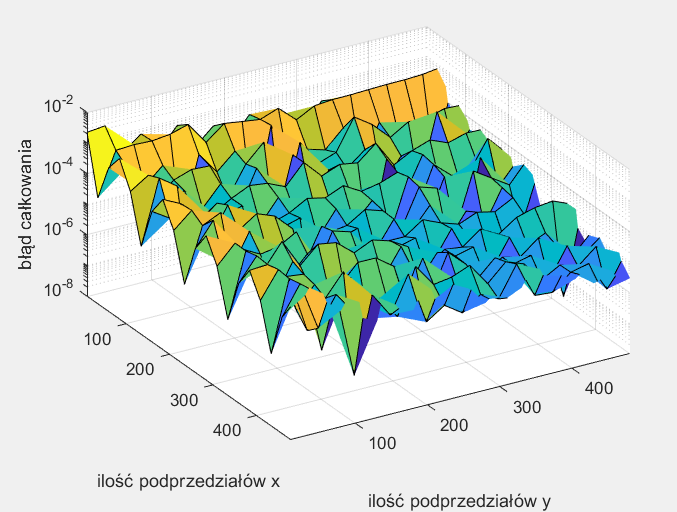
\includegraphics[width=9cm]{3D_3d.png}
    \caption{B\l ędy dla rosnącej liczby podprzedzia\l \'ow po odpowiednich wsp\'o\l rzędnych}
\end{figure}

Jak wida\'c, wystarczy aby liczba podprzedzia\l \'ow by\l a ma\l a dla jednego z wymiar\'ow by b\l ąd by\l  \ o wiele większy.
Ponadto na tym wykresie nadal wida\'c, \.ze b\l ąd maleje dla coraz większej ilo\'sci przedzia\l \'ow.
Aby lepiej zobrazowa\'c ten efekt poni\.zej umieszczony zosta\l \ ten wykres widziany od g\'ory.

\begin{figure}[H]
    \centering
    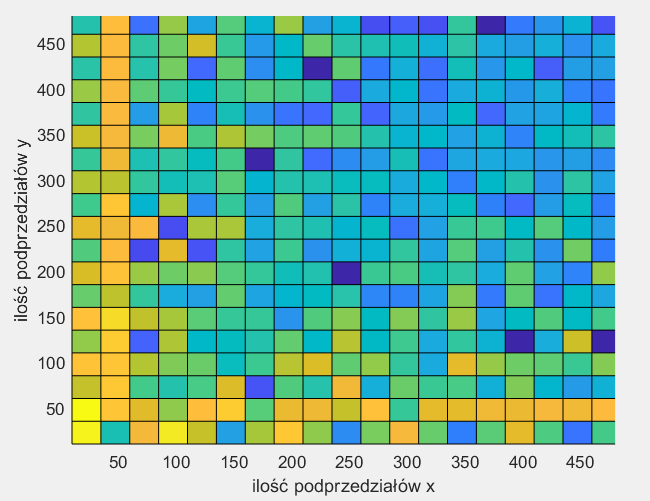
\includegraphics[width=8.5cm]{3D_2d.png}
    \caption{B\l ędy dla rosnącej liczby podprzedzia\l \'ow po odpowiednich
    wsp\'o\l rzędnych pokazany  od g\'ory}
\end{figure}
Im ja\'sniejszy jest kolor tym większe są b\l ędy, dzięki czemu wida\'c,
\.ze kolor najja\'sniejszy jest najbli\.zej osi wykresu czyli tam gdzie 
ilo\'s\'c podprzedzia\l \'ow jest najmniejsza. \\ 
Wszystkie testy wykonane w tym punkcie dowodzą r\'ownie\.z, \.ze funkcja 
dla odpowiednio du\.zej ilo\'sci podprzedzia\l \'ow wyznacza ca\l kę 
funkcji dw\'och zmiennych z akceptowalną dok\l adno\'scią.

\section{Podsumowanie}
Podsumowując, powy\.zsze eksperymenty pokaza\l y u\.zyteczno\'s\'c funkcji 
obliczającej tytu\l owe zadanie. Zosta\l o pokazane, \.ze: \\
\begin{itemize}
        \item
            Metoda u\.zyta w zadaniu do przekszta\l cenia obszaru ca\l kowania
            jest poprawna.
        \item
            Program dzia\l a dobrze dla wielomian\'ow stopnia mniejszego 
            ni\.z 4, oraz optymalne jest u\.zywanie tylko jednego podprzedzia\l u
            do ca\l kowania tych funkcji.
        \item
            Dla wystarczającej liczby podprzedzia\l \'ow program z zadowalającą
            dok\l adno\'scią oblicza ca\l ki bardziej skomplikowanych funkcji.
            Ponadto im więcej podprzedzia\l \'ow u\.zyjemy, tym większa będzie 
            ta dok\l adno\'s\'c. Wystarczy jednak aby w jednym wymiarze 
            by\l o niewystarczająco podprzedzia\l \'ow aby obliczenia sta\l y
            się do\'s\'c niedok\l adne.
        \item
            Metoda Simpsona daje dok\l adniejsze wyniki ni\.z metoda trapez\'ow.
            Co więcej na bazie tej dok\l adno\'sci mo\.zemy wnioskowa\'c, \.ze 
            jest to metoda rzędu o jeden wy\.zszego. Czas dzia\l ania programu
            dla metody Simpsona jest jednak istotnie d\l u\.zszy.

\end{itemize}


\end{document}
